\section{Ejercicio 8}

Se pedía implementar un scheduler, \texttt{SchedRR2}, con modalidad Round-Robin
y que no permitiera migrar los procesos entre núcleos. El CPU correspondiente a
cada proceso es seleccionado durante su carga, correspondiendo en cada caso
aquel con menor cantidad total de procesos activos.

\subsection{Implementación del scheduler}

Al igual que en ejercicios anteriores, el constructor del scheduler recibe por
parámetro la cantidad de \emph{cores} y el tiempo del \emph{quantum}
correspondiente a cada uno de ellos. Estos valores son almacenados, guardando
por duplicado la duración de los \emph{quantums} para luego poder ir
decrementando una de las copias. Durante la inicialización, además, se crean
estas estructuras adicionales: un vector para almacenar la cantidad de
procesos que se están ejecutando en cada procesador, un vector de vectores que
contiene los PIDs de cada uno de ellos, y un vector con las colas de
\emph{ready} correspondientes a cada \emph{core}.

Al cargar un proceso en el scheduler, se utiliza el primero de los vectores
mencionados para seleccionar el núcleo que tenga menos procesos activos. Luego
el proceso recién cargado se agrega en la cola de \emph{ready} del \emph{core}
y en su lista de tareas activas, y se incrementa en uno su contador de
procesos.

Cuando se produce una llamada a la función \texttt{tick}, es decir, cuando se
produce un \emph{tick} del reloj de algún CPU y el \emph{scheduler} es
invocado, se realizan diferentes acciones según cuál haya sido la actividad de
la CPU durante el \emph{quantum} anterior.

En varias ocasiones se relizan llamadas a la función auxiliar \texttt{next},
que desencola la próxima tarea de la cola de \emph{ready} de una CPU y
devuelve su PID, en caso de que esto sea posible, y en caso contrario devuelve
el PID de la tarea \emph{idle}. Además, esta función reinicia el contador de
tiempo de
\emph{quantum} restante del CPU a su valor inicial.

\begin{enumerate}
    \item Si el proceso anterior consumió todo el ciclo de CPU, puede tratarse
    de la tarea \emph{idle}, en cuyo caso simplemente se realiza una llamada a
    \texttt{next}, o bien puede tratarse de otra tarea en ejecución. En este
    caso se chequea si aún sobra tiempo del \emph{quantum} actual. De ser así,
    se decrementa en uno el contador de tiempo restante y se decide que siga
    ejecutando el mismo proceso. En caso contrario, se desaloja al proceso
    utilizando la función \texttt{next} y se lo vuelve a colocar en la cola de
    \emph{ready}.
    \item Si el proceso anterior realizó una llamada bloqueante, simplemente se
    lo desaloja con la función \texttt{next}. Cuando el proceso se desbloquee,
    la función \texttt{unblock} se encargará de hacerlo volver a la cola de
    \emph{ready}.
    \item Si el proceso anterior acaba de terminar, entonces se lo reemplaza por
    el proceso siguiente ejecutando \texttt{next} y, además, se lo elimina de
    las lista de tareas activas del CPU donde estaba registrado. También se
    decrementa en uno el contador de tareas activas de este CPU.
\end{enumerate}

\subsection{Experimentación}

Se pedía realizar una comparación entre este criterio de \emph{scheduling}
y otro que sí permitiera la migración entre procesadores. Con este fin, se
comparó el \emph{scheduler} obtenido con el desarrollado anteriormente en el
Ejercicio 4 (\texttt{SchedRR}).

Para comparar los resultados producidos por ambos \emph{schedulers}, se
plantearon tres ejemplos de escenarios reales; en dos de ellos, uno de los
modelos resultó superior al otro, mientras que en el otro los resultados
dependen de las métricas consideradas. Los escenarios ideados fueron los
siguientes:

\begin{enumerate}
    \item En una máquina con dos CPUs, se ejecuta una serie de procesos, cada
    uno de ellos con un tiempo total de ejecución breve. Esta situación
    produce dos aspectos a tener en cuenta: por un lado, el tiempo insumido
    por la migración de los procesos se vuelve apreciable en comparación con
    el utilizado para su ejecución; este inconveniente se presenta a menudo en
    sistemas reales, donde para evitarlo muchas veces se establece una cota
    mínima para la antigüedad de un proceso antes de poder
    migrarlo\footnote{Milojičić, Dejan S. et al., \emph{Process migration}
    (ACM Computing Surveys, 2000)}. Por otra parte, el hecho de que la
    duración de todas las tareas sea similar genera una distribución
    equilibrada entre las cargas de cada núcleo incluso al utilizar el
    \emph{scheduler} sin migración, entendiendo como carga de un núcleo el
    tiempo total de ejecución de los procesos asignados al mismo.

    Estas circunstancias producen que las ventajas que puede presentar un
    \emph{scheduler} con migración (balancear la carga entre los procesadores,
    evitando que uno de ellos quede ocioso mientras hay tareas por ejecutar)
    se vuelvan poco significativas con respecto al costo que tiene realizar la
    migración. De esta forma, utilizar este tipo de \emph{scheduler}
    produce una caída en el rendimiento general del sistema, afectando
    negativamente métricas como el \emph{waiting-time} y el \emph{turnaround}
    de los procesos. Por lo tanto, en este contexto es claramente preferible
    un algoritmo de \emph{scheduling} sin migración.

    Se consideró un costo para la migración de 6 unidades de tiempo, y un
    \emph{quantum} para ambos núcleos de 8 unidades de tiempo. Las siete
    tareas consideradas utilizan el CPU sin bloquearse y tienen duraciones de
    entre 9 y 12 unidades de tiempo.

    \item También en una máquina con dos CPUs, se ejecuta una tarea que hace
    un uso intensivo del CPU y varias tareas interactivas, es decir, que hacen
    un gran uso de entrada/salida. Aquí el \emph{scheduler} sin migración
    asignará a la mitad de las tareas interactivas el mismo
    \emph{core} que a la tarea intensiva, provocando una disminución en la 
    \emph{latencia} o tiempo de respuesta de las mismas. El \emph{scheduler}
    con migración, en cambio, permitirá que, mientras la tarea intesiva
    utiliza un procesador, cualquiera de las tareas interactivas pueda ocupar
    el otro, obteniendo así mejores resultados para esta métrica.

    No obstante, en el caso del algoritmo sin migración, se obtuvieron mejores
    resultados para el \emph{turnaround} y el \emph{waiting-time}. Esto se
    debe a que las tareas interactivas que resultan asignadas al \emph{core}
    que no ejecuta la tarea intensiva se ven muy beneficiadas por este hecho,
    generando una disminución importante en los promedios de estas métricas.
    Cabe destacar, sin embargo, que incluso a pesar de estos resultados, las
    mejores métricas alcanzadas por algunas de las tareas interactivas tienen
    como contrapeso un peor rendimiento por parte de las otras, lo cual tiene
    un impacto negativo en la justicia del algoritmo. Es importante tener en
    cuenta además que en el caso de tareas interactivas, lo que se desea es
    minimizar el tiempo de respuesta al usuario para que el funcionamiento del
    sistema resulte fluido; por lo tanto, en este escenario la \emph{latencia}
    podría resultar una métrica más relevante que el \emph{turnaround} o el
    \emph{waiting-time}.

    El costo de la migración entre \emph{cores} se estableció en 4 unidades de
    tiempo, y los \emph{quantums} de ambos núcleos en 8 unidades de tiempo. La
    tarea intensiva utiliza el CPU durante 40 unidades de tiempo, mientras que
    las seis tareas interactivas se bloquean cada una tres veces durante 5
    unidades de tiempo.

    \item Como ejemplo en el que resulta claramente conveniente el uso de
    \emph{scheduling} con migración, se pensó en un sistema, también con dos
    núcleos, donde los procesos llegan de forma tal que resultan distribuidos
    de una forma poco equilibrada entre los CPUs. En este caso, al emplear el
    algoritmo sin migración, uno de los dos procesadores queda ocioso mientras
    mientras todavía hay procesos pendientes, asignados de forma exclusiva al
    otro núcleo. El algoritmo con migración permite mitigar este defecto
    redistribuyendo la carga cada vez que cambia la tarea en ejecución. Cabe
    mencionar que, si bien la posibilidad de rebalancear la carga es uno de
    las grandes ventajas que proporciona la migración de procesos, podría
    mejorarse el rendimiento de un \emph{scheduler} sin migración si se
    utilizara una estrategia más inteligente a la hora de distribuir los
    procesos durante su carga. Las métricas utilizadas para comparar los dos
    algoritmos fueron el \emph {waiting-time} y el \emph{turnaround},
    obteniendo en ambos casos mejores resultados con el \emph{scheduler} con
    migración.

    Se consideró un costo para la migración entre núcleos de 4 unidades de
    tiempo y \emph{quantums} para ambos \emph{cores} de 8 unidades de tiempo.
    Se ejecutan tres tareas largas, de 15, 18 y 12 unidades de tiempo, y tres
    tareas cortas, con duraciones de 4, 3 y 6 unidades de tiempo, que llegan
    al procesador de manera intercalada.
\end{enumerate}

A continuación se muestran los gráficos y las mediciones obtenidas en ambas
implementaciones para los lotes de tareas \texttt{ej8\_1}, \texttt{ej8\_2} y
\texttt{ej8\_3}, realizados según los tres escenarios recién propuestos.

\begin{figure}[H]
    \begin{center}
        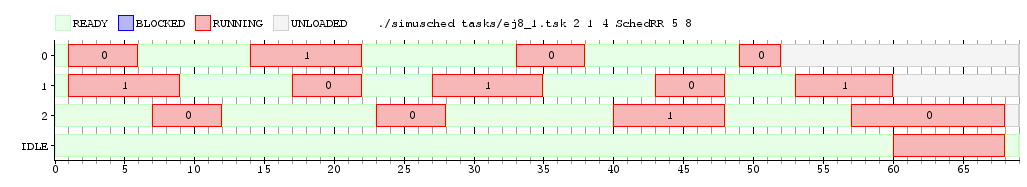
\includegraphics[width=1\columnwidth]{imagenes/ej8_1_rr.png}
        \caption{Escenario 1 en \emph{scheduler} con migración (\texttt{SchedRR})}
    \end{center}
\end{figure}

\begin{figure}[H]
    \begin{center}
        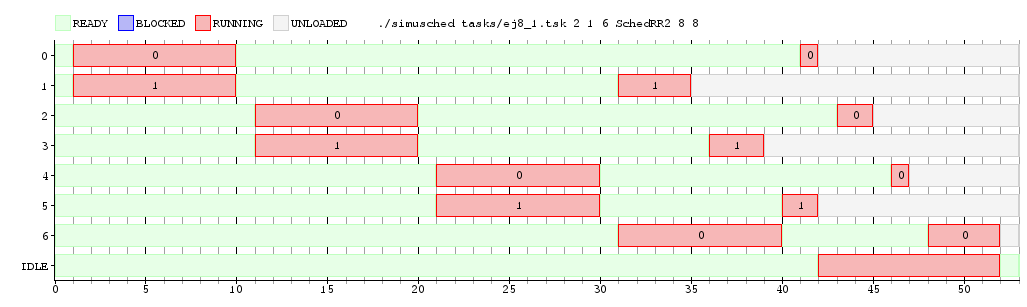
\includegraphics[width=1\columnwidth]{imagenes/ej8_1_rr2.png}
        \caption{Escenario 1 en \emph{scheduler} sin migración (\texttt{SchedRR2})}
    \end{center}
\end{figure}

\begin{table}[H]
    \begin{center}
        \begin{tabular}{|c|c|c|c|}
            \hline
            \textbf{Scheduler}                 & \textbf{Waiting-time} & \textbf{Turnaround} \\ \hline
            \texttt{SchedRR} (con migración)   & 39.429                & 50.857 \\
            \texttt{SchedRR2} (sin migración)  & 31.714                & 43.143 \\ \hline
        \end{tabular}
        \caption{Tiempos promedio para el Escenario 1, para cada \emph{scheduler}}
    \end{center}
\end{table}


\begin{figure}[H]
    \begin{center}
        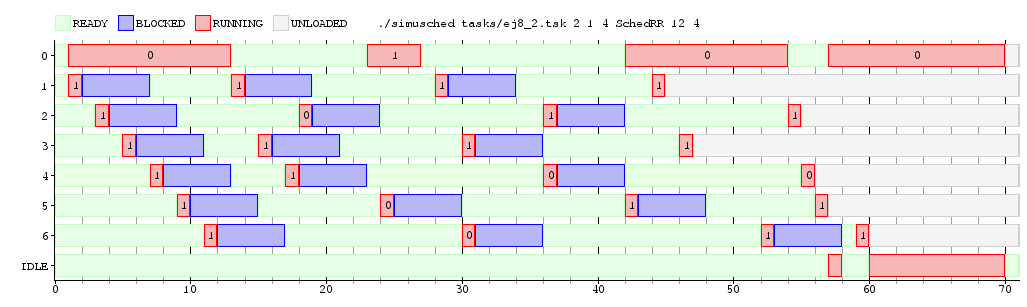
\includegraphics[width=1\columnwidth]{imagenes/ej8_2_rr.png}
        \caption{Escenario 2 en \emph{scheduler} con migración (\texttt{SchedRR})}
    \end{center}
\end{figure}

\begin{figure}[H]
    \begin{center}
        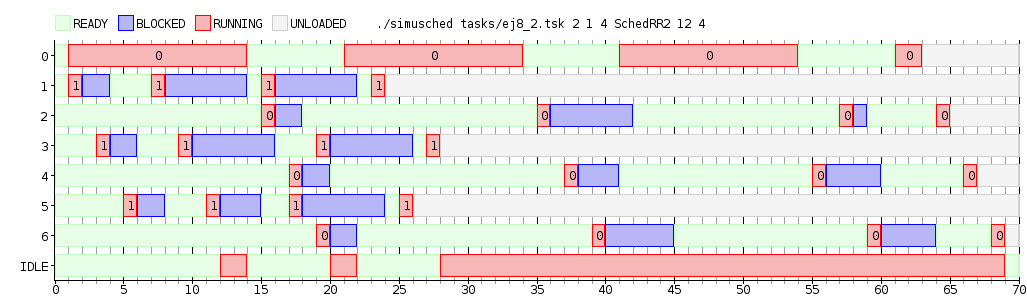
\includegraphics[width=1\columnwidth]{imagenes/ej8_2_rr2.png}
        \caption{Escenario 2 en \emph{scheduler} sin migración (\texttt{SchedRR2})}
    \end{center}
\end{figure}

\begin{table}[H]
    \begin{center}
        \begin{tabular}{|c|c|c|c|}
            \hline
            \textbf{Scheduler}                 & \textbf{Latencia} & \textbf{Waiting-time} & \textbf{Turnaround} \\ \hline
            \texttt{SchedRR} (con migración)   & 5.143             & 37.286                & 59.429 \\
            \texttt{SchedRR2} (sin migración)  & 7.857             & 26.286                & 48.429 \\ \hline
        \end{tabular}
        \caption{Tiempos promedio para el Escenario 2, para cada \emph{scheduler}}
    \end{center}
\end{table}


\begin{figure}[H]
    \begin{center}
        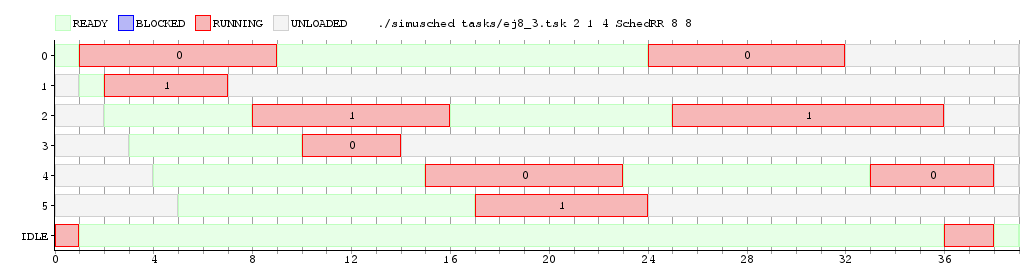
\includegraphics[width=1\columnwidth]{imagenes/ej8_3_rr.png}
        \caption{Escenario 3 en \emph{scheduler} con migración (\texttt{SchedRR})}
    \end{center}
\end{figure}

\begin{figure}[H]
    \begin{center}
        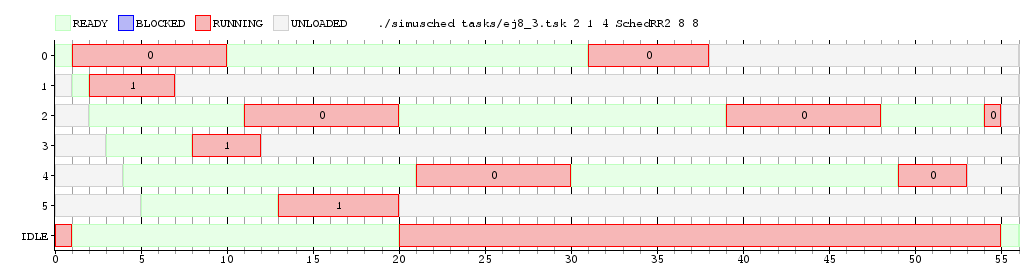
\includegraphics[width=1\columnwidth]{imagenes/ej8_3_rr2.png}
        \caption{Escenario 3 en \emph{scheduler} sin migración
        (\texttt{SchedRR2}). Notar cómo el \emph{core} 1 queda ocioso
        rápidamente, resultando en una mala distribución de la carga que
        repercute negativamente en el rendimiento.}
    \end{center}
\end{figure}

\begin{table}[H]
    \begin{center}
        \begin{tabular}{|c|c|c|c|}
            \hline
            \textbf{Scheduler}                 & \textbf{Waiting-time} & \textbf{Turnaround} \\ \hline
            \texttt{SchedRR} (con migración)   & 12                    & 22.667 \\
            \texttt{SchedRR2} (sin migración)  & 17.667                & 28.333 \\ \hline
        \end{tabular}
        \caption{Tiempos promedio para el Escenario 3, para cada \emph{scheduler}}
    \end{center}
\end{table}
